\documentclass[border=6pt]{standalone}
\usepackage{tikz}
\usetikzlibrary{arrows.meta,calc}
\begin{document}
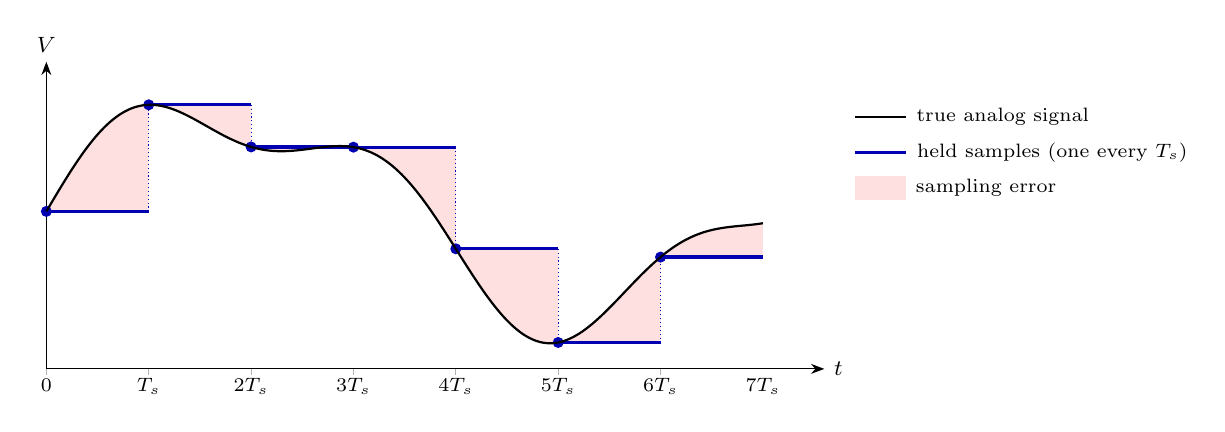
\begin{tikzpicture}[>=Stealth,font=\small,x=1.3cm,y=1cm,
 declare function={v(\t)=2.0+1.3*sin(deg(\t*0.9))+0.45*sin(deg(\t*2.3));}]
\draw[->] (0,0) -- (7.6,0) node[right,font=\footnotesize]{$t$};
\draw[->] (0,0) -- (0,3.9) node[above,font=\footnotesize]{$V$};
% held samples (zero-order hold): sample at k*Ts, hold until (k+1)*Ts
\foreach \k in {0,...,6} {
  \pgfmathsetmacro{\y}{v(\k)}
  \pgfmathsetmacro{\yn}{v(\k+1)}
  \fill[red!12] plot[domain=\k:\k+1,samples=20] (\x,{v(\x)}) -- (\k+1,\y) -- (\k,\y) -- cycle;
  \draw[very thick,blue!70!black] (\k,\y) -- (\k+1,\y);
  \ifnum\k<6 \draw[blue!70!black,densely dotted] (\k+1,\y) -- (\k+1,\yn); \fi
  \fill[blue!70!black] (\k,\y) circle (2pt);
  \draw[gray!60] (\k,0) -- (\k,-0.08);
}
\draw[thick] plot[domain=0:7,samples=120,smooth] (\x,{v(\x)});
\foreach \k/\l in {0/0,1/$T_s$,2/$2T_s$,3/$3T_s$,4/$4T_s$,5/$5T_s$,6/$6T_s$,7/$7T_s$} \node[below,font=\scriptsize] at (\k,0) {\l};
% legend
\begin{scope}[shift={(7.9,3.2)}]
\draw[thick] (0,0) -- (0.5,0) node[right,font=\scriptsize]{true analog signal};
\draw[very thick,blue!70!black] (0,-0.45) -- (0.5,-0.45) node[right,font=\scriptsize,black]{held samples (one every $T_s$)};
\fill[red!12] (0,-1.05) rectangle (0.5,-0.75); \node[right,font=\scriptsize] at (0.5,-0.9) {sampling error};
\end{scope}
\end{tikzpicture}
\end{document}
